\flushbottom




%%=============================================================================
%%=============================================================================
\chapter{Introduction}
\label{chapter_ode_introduction}




%%=============================================================================
\section{Basic Concepts}

A \textit{differential equation} is an equation involving a function,
its derivatives, and independent variables.  If there is only one 
independent variable, then it is an 
\textit{ordinary differential equation}.
\index{differential equations!ordinary}
Otherwise it is a 
\textit{partial differential equation}.
\index{differential equations!partial}
\[
y''(x) + y(x) = 0
\]
is an ordinary differential equation.
\[
\frac{ \partial^2 \psi}{\partial x^2} + \frac{ \partial^2 \psi}{\partial y^2} = 0
\]
is a partial differential equation for $\psi(x,y)$.
Identities such as 
\[
\frac{\dd}{\dd x} \left( y^2(x) \right) = 2 y(x) y'(x), 
\quad \mathrm{and} \quad
\frac{\dd y}{\dd x} \frac{\dd x}{\dd y} = 1
\]
are not differential equations.



Differential equations are useful in modelling many scientific problems.
Consider some physical process that evolves in time - like an object 
undergoing radioactive decay, the motion of a pendulum, or the 
vibration of a guitar string.  
For the pendulum, the position and velocity determine its \textit{state}.
If we were concerned only with the amount of material in the decaying object,
then its mass describes its state.  To describe the state of the guitar
string, we would have to specify its position and velocity at each point
along the string.  

The set of all possible states of a process is its \textit{phase
  space}.  For the decaying mass, the phase space is the set of
non-negative real numbers $\mathbb{R}^{0+}$.  For the pendulum, the
angle $\theta$ from vertical determines its position.  The angular velocity
$\dot{\theta}$ determines the velocity.  The phase space is $\mathbb{R}^2$
where the horizontal axis measures $\theta$ and the vertical axis measures
$\dot{\theta}$.  One could also represent $\theta$ as a cyclic coordinate.  In 
this case the phase space is the surface of a cylinder.  The axes of
these two representations are shown in 
Figure~\ref{figure pendulum phase space}.
Since there are an infinite number of points along the guitar string,
its phase space has infinite dimension.


\begin{figure}[tb!]
  \begin{center}
    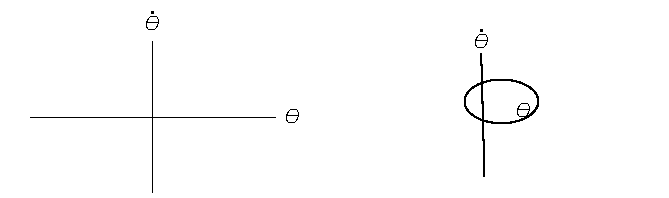
\includegraphics[width=0.5\textwidth]{ode/introduction/pendulum_phase_space}
  \end{center}
  \caption{Two phase spaces for the pendulum.}
  \label{figure pendulum phase space}
\end{figure}


In order to model a process with differential equations it must be 
\textit{deterministic}
\index{deterministic} 
and \textit{differentiable}.  Deterministic means that all past and future
states of the process are determined by its present state.  Each of the 
three examples under consideration are deterministic.  A process is 
differentiable if the phase space is a 
differentiable manifold\footnote{If you don't like the sound of 
``differentiable manifold'', say ``smooth surface'' instead.}
and the evolution of the process is described by differentiable functions.  
Each of our examples are differentiable.

As a side note: the decaying object is deterministic and differentiable 
only when we consider the mass to be continuous.  The object is made up
of atoms.  When individual atoms decay, the mass jumps discontinuously.
With this interpretation, the phase space is the set of points 
$\{ n M : n \in \mathbb{Z}, n \geq 0\}$ where $M$ is the mass of an atom.  The 
phase space is not a differentiable manifold, so the process is not 
differentiable.  Since we don't know exactly when the atoms decay, 
the process is not deterministic.  However, since there are a lot of atoms
it is a good approximation to consider the mass to be continuous.


In addition to being deterministic and differentiable, the phase space of 
a process must be \textit{finite dimensional} in order to be modeled by 
ordinary differential equations.  The decaying mass and the pendulum 
may both be modeled by ordinary differential equations.
Many infinite dimensional processes like the guitar string, may be modeled 
with partial differential equations.


%% CONTINUE HERE


%%=============================================================================
\section{Notation}

The \textit{order} of a differential equation is the order of the highest 
derivative.
\index{order!of a differential equation}
\index{differential equations!order}
The following equations for $y(x)$ are first, second and third order, 
respectively.
\begin{itemize}
\item $y' = x y^2$
\item $y'' + 3 x y' + 2 y = x^2$
\item $y''' = y'' y$
\end{itemize}

The \textit{degree} of a differential equation is the highest power of 
the highest
\index{degree!of a differential equation}
\index{differential equations!degree}
derivative in the equation.  The following equations are first, second 
and third degree, respectively.
\begin{itemize}
\item $y' - 3 y^2 = \sin x$
\item $(y'')^2 + 2 x \cos y = \e^x$
\item $(y')^3 + y^5 = 0$
\end{itemize}
An equation is said to be \textit{linear} if it is linear in the dependent 
variable.
\index{linear differential equations}
\index{differential equations!linear}
\begin{itemize}
\item $y'' \cos x + x^2 y = 0$ is a linear differential equation.
\item $y' + x y^2 = 0$ is a nonlinear differential equation.
\end{itemize}

A differential equation is \textit{homogeneous} if it has no terms that 
are functions of the
\index{homogeneous differential equations}
\index{differential equations!homogeneous}
independent variable alone.  Thus an \textit{inhomogeneous} equation is one in
\index{inhomogeneous differential equations}
\index{differential equations!inhomogeneous}
which there are terms that are functions of the independent variables alone.
\begin{itemize}
\item $y'' + x y + y = 0$ is a homogeneous equation.
\item $y' + y + x^2 = 0$ is an inhomogeneous equation.
\end{itemize}


A first order differential equation may be written in terms of differentials.
Recall that for the function $y(x)$ the differential $\dd y$ is defined
$\dd y = y'(x)\,\dd x$.  Thus the differential equations
\[
y' = x^2 y \quad \mathrm{and} \quad y' + x y^2 = \sin(x)
\]
can be denoted:
\[
\dd y = x^2 y \,\dd x \quad \mathrm{and} \quad 
\dd y + x y^2 \,\dd x = \sin(x) \,\dd x.
\]


A \textit{solution} of a differential equation is a function which when 
substituted into the equation yields an identity.  For example,
$y = x \ln |x|$ is a solution of 
\[
y' - \frac{y}{x} = 1.
\]
We verify this by substituting it into the differential equation.
\[
\ln |x| + 1 - \ln |x| = 1
\]

We can also verify that $y = c \e^x$ is a solution of $y'' - y  = 0$
for any value of the parameter $c$.
\[
c \e^x - c \e^x = 0
\]






%%=============================================================================
\section{Example Problems}



In this section we will discuss physical problems that lead 
to differential equations.


%%---------------------------------------------------------------------------
\subsection{Growth and Decay}



\begin{Example}
  Consider a culture of bacteria in which each bacterium divides 
  once per hour.  Let $n(t) \in \mathbb{N}$ denote the 
  population, let $t$ denote the time in hours and let $n_0$ be the 
  population at time $t = 0$.  The population doubles every hour.  Thus 
  for integer $t$, the population is $n_0 2^t$.  Figure~\ref{figure bacteria1}
  shows two possible populations when there is initially a single 
  bacterium.  In the first plot, each of the bacteria divide at times
  $t = m$ for $m \in \mathbb{N}$.  In the second plot, they divide at 
  times $t = m - 1/2$.  For both plots the population is $2^t$ for 
  integer $t$.

  \begin{figure}[tb!]
    \begin{center}
      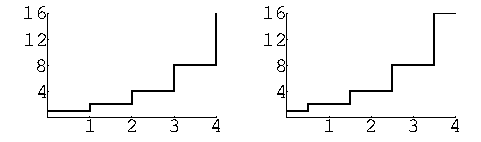
\includegraphics[width=0.6\textwidth]{ode/introduction/bacteria1}
    \end{center}
    \caption{The population of bacteria.}
    \label{figure bacteria1}
  \end{figure}

  We model this problem by considering a continuous population 
  $y(t) \in \mathbb{R}$ which approximates the discrete population.
  In Figure~\ref{figure bacteria8} we first show the population
  when there is initially 8 bacteria.  The divisions of bacteria is 
  spread out over each one second interval.   For integer $t$, the 
  population is $8 \cdot 2^t$.  Next we show the population with a plot of 
  the continuous function $y(t) = 8 \cdot 2^t$.  We see that $y(t)$ is a 
  reasonable approximation of the discrete population.  
  
  \begin{figure}[tb!]
    \begin{center}
      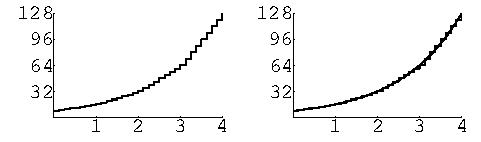
\includegraphics[width=0.6\textwidth]{ode/introduction/bacteria8}
    \end{center}
    \caption{The discrete population of bacteria and a continuous 
      population approximation.}
    \label{figure bacteria8}
  \end{figure}

  In the discrete problem, the growth of the population is proportional 
  to its number; the population doubles every hour.  For the continuous
  problem, we assume that this is true for $y(t)$.  We write this as an 
  equation:
  \[
  y'(t) = \alpha y(t).
  \]
  That is, the rate of change $y'(t)$ in the population is proportional
  to the population $y(t)$, (with constant of proportionality $\alpha$).
  We specify the population at time $t = 0$ with the initial condition:
  $y(0) = n_0$.  Note that $y(t) = n_0 \e^{\alpha t}$ satisfies the problem:
  \[
  y'(t) = \alpha y(t), \quad y(0) = n_0.
  \]
  For our bacteria example, $\alpha = \ln 2$.
\end{Example}


\begin{Result}
  A quantity $y(t)$ whose growth or decay is proportional to $y(t)$
  is modelled by the problem:
  \[
  y'(t) = \alpha y(t), \quad y(t_0) = y_0.
  \]
  Here we assume that the quantity is known at time $t = t_0$.
  $\e^\alpha$ is the factor by which the quantity grows/decays in unit time.
  The solution of this problem is
  $y(t) = y_0 \e^{\alpha (t - t_0)}$.
\end{Result}



\begin{Example}
  Consider a body of radioactive material.  Suppose that we 
  know from physical principles that the rate of decay is proportional to the 
  mass of the body.  At noon the body is 5 grams; by 1:00 PM  it has
  decreased to 4 grams.  When will it be 1 gram?

  Let $y(t)$ be the mass of the body where $t$ measures time in hours and 
  let noon be $t = 0$.  This problem is modelled by:
  \[
  y'(t) = \alpha y(t), \quad y(0) = 5,
  \]
  which has the solution $y(t) = 5 \e^{\alpha t}$.  We substitute in our measurement
  at 1:00 PM to determine the constant of proportionality.
  \begin{gather*}
    4 = 5 \e^{\alpha}
    \\
    \alpha = \ln(4 / 5)
  \end{gather*}
  Thus the solution is $y(t) = 5 (4/5)^t$.  We substitute in $y(t) = 1$ to 
  determine when the body will be 1 gram.
  \begin{gather*}
    1 = 5 (4/5)^t
    \\
    0 = \ln 5 + t \ln(4/5)
    \\
    t = - \frac{ \ln 5 }{ \ln(4/5) } \approx 7.21
  \end{gather*}
  Thus we see that there will be 1 gram remaining at about 7:13 PM.
\end{Example}





%%---------------------------------------------------------------------------
\subsection{1-Dimensional Trajectory Motion}

Consider the vertical motion of an object under the force of gravity.
Let $x$ be the elevation of the object.  The position $x$ and velocity
$\dot{x}$ define its state.  If we neglect air friction, then the 
object experiences an acceleration of $-g$ due to gravity\footnote{
We also assume that the change in the elevation of the object is small enough
to consider the gravitational acceleration to be constant.}.
We write this as a differential equation.
\[
\ddot{x} = - g
\]
We can solve the differential equation by twice integrating with respect 
to $t$.  We will do this in two different ways.  First we take 
indefinite integrals to obtain
\[
x(t) = - \frac{g}{2} t^2 + c_1 t + c_2,
\]
where $c_1$ and $c_2$ are constants of integration.
Suppose that the object has position $x_0$ and velocity $v_0$ at time $t_0$.
We can apply these two constraints, known as \textit{intial conditions},
to determine the constants of integration.
\begin{gather*}
  x(t_0) = x_0 \quad \Rightarrow \quad - \frac{g}{2} t_0^2 + c_1 t_0 + c_2 = x_0
  \\
  \dot{x}(t_0) = v_0 \quad \Rightarrow \quad -g t_0 + c_1 = v_0
  \\
  x(t) = - \frac{g}{2} t^2 + (g t_0 + v_0) t 
  - \frac{g}{2} t_0^2 - t_0 v_0 + x_0
\end{gather*}
\begin{equation}
  \label{equation 1D trajectory solution}
  x(t) = - \frac{g}{2} (t - t_0)^2 + v_0 (t - t_0) + x_0
\end{equation}

Another approach is to take definite integrals from $t_0$ to $t$.
\begin{gather*}
  \ddot{x} = - g
  \\
  \int_{t_0}^t \ddot{x}(\tau) \,\dd \tau = \int_{t_0}^t -g \,\dd \tau 
  \\
  \dot{x}(t) - \dot{x}(t_0) = - g (t - t_0)
  \\
  \int_{t_0}^t (\dot{x}(\tau) - v_0) \,\dd \tau = \int_{t_0}^t -g (\tau - t_0) \,\dd \tau 
  \\
  x(t) - x(t_0) - v_0 (t - t_0) = - \frac{g}{2} (t - t_0)^2
  \\
  x(t) = - \frac{g}{2} (t - t_0)^2 + v_0 (t - t_0) + x_0
\end{gather*}
We obtain the same result either way.  For the latter method, the initial
conditions are introduced as we evaluate the definite integrals.

There are a number of ways to plot the motion of the trajectory.  First 
consider an object dropped at $t = 0$ from an initial height of $x_0$.
In the first plot in Figure~\ref{figure trajectory 1d tx} we show the 
elevation versus time.  Then consider an object projected upward at $t = 0$
with an initial velocity of $v_0$.  These trajectories are shown in the
second plot.

\begin{figure}[tb!]
  \begin{center}
    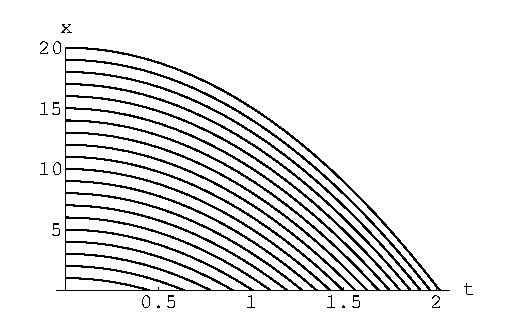
\includegraphics[width=0.49\textwidth]{ode/introduction/trajectory_1d_tx_x0}
    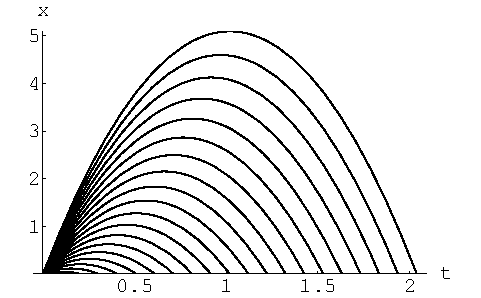
\includegraphics[width=0.49\textwidth]{ode/introduction/trajectory_1d_tx_v0}
  \end{center}
  \caption{Trajectories of objects dropped from an initial height and 
    projected upward from zero height.}
  \label{figure trajectory 1d tx}
\end{figure}

We can also plot these trajectories in phase space.  (See 
Figure~\ref{figure trajectory 1d xxd}.)  These plots show the evolution of the 
state of the object.

\begin{figure}[tb!]
  \begin{center}
    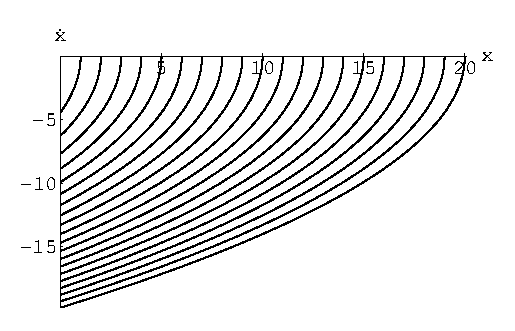
\includegraphics[width=0.49\textwidth]{ode/introduction/trajectory_1d_xxd_x0}
    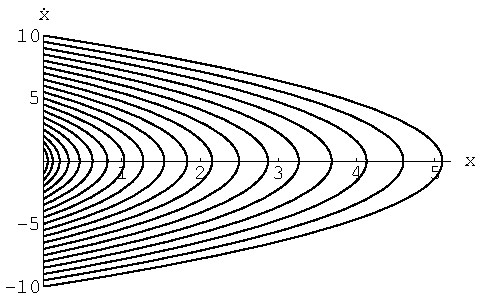
\includegraphics[width=0.49\textwidth]{ode/introduction/trajectory_1d_xxd_v0}
  \end{center}
  \caption{The trajectories plotted in phase space.}
  \label{figure trajectory 1d xxd}
\end{figure}


Note that the time factors in the solution subject to the initial conditions 
(Equation~\ref{equation 1D trajectory solution})
all appear as $(t - t_0)$.  This is not mere coincidence.  The equation
of motion $\ddot{x} = - g$ is \textit{shift invariant} with respect to $t$.
\index{shift invariant}
This means that the equation is unchanged under the transformation 
$t \to t - t_0$.   We can state this in physical terms: the motion of the 
object does not depend on the starting time.  The object will fall in 
the same manner whether we drop it today, tomorrow or next week.  Thus, 
without loss of generality, we can take the starting time to be $t = 0$.
In this case the solution is
\[
x(t) = - \frac{g}{2} t^2 + v_0 t + x_0
\]
If we change the starting time to $t = 42$, we just make the 
substitution $t \to t - 42$ to obtain the solution for the new 
starting time.
\[
x(t) = - \frac{g}{2} (t - 42)^2 + v_0 (t - 42) + x_0
\]



%%---------------------------------------------------------------------------
\subsection{2-Dimensional Trajectory Motion}

Consider the 2-D motion of an object under the force of gravity.
Let $(x,y)$ be the position of the object.  The position $(x,y)$ and velocity
$(\dot{x}, \dot{y})$ define its state.  The 
object experiences an acceleration of $-g$ in the vertical direction 
due to gravity.  There is no applied force in the horizontal direction.
We write these relations as differential equations.
\[
\ddot{x} = - g, \quad \ddot{y} = 0
\]

\begin{Exercise}
  \label{exercise hunter monkey}
  A hunter aims his rifle exactly at a monkey hanging from a tree branch.
  At the same time the hunter pulls the trigger, the monkey lets go of
  the branch.  Does the bullet hit the monkey?  Solve the differential
  equations of motion to find out.
  
  \hintsolution{hunter monkey}
\end{Exercise}




%%---------------------------------------------------------------------------
\subsection{Mass on a Spring}


\begin{figure}[tb!]
  \begin{center}
    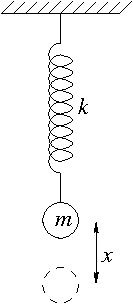
\includegraphics[width=0.15\textwidth]{ode/introduction/mass_on_spring}
  \end{center}
  \caption{A mass on a spring.}
  \label{figure mass on spring}
\end{figure}

Consider the vertical motion of a ball of mass $m$ suspended from an 
ideal spring\footnote{An ideal spring is massless and obeys Hooke's law.}.  
(See Figure~\ref{figure mass on spring}.)  Let $x$ be the displacement 
from the equilibrium position.  Hooke's law 
\index{Hooke's law} 
states that the force from the spring is directly proportional to this 
displacement.
\[
\mathrm{force} = - k \ \mathrm{displacement}
\]
$k$ is called the spring constant.  The force applied to the mass is equal
to the derivative of its momentum $m \dot{x}$.  We use this to obtain a 
differential equation for the motion.
\begin{gather*}
  \frac{\dd}{\dd t}(m \dot{x}) = - k x
  \\
  \ddot{x} + \frac{k}{m} x = 0
\end{gather*}

Now we make the unmotivated substitution $\omega_0 := k / m$.  The equation becomes
\begin{equation}
  \label{ddot x + w02 x = 0}
\ddot{x} + \omega_0^2 x = 0.
\end{equation}

\begin{Exercise}
  \label{exercise mass on spring solutions}
  Verify that both
  \[
  x = a \cos( \omega_0 t ) + b \sin( \omega_0 t )
  \]
  and
  \[
  x = A \sin( \omega_0 t + \phi )
  \]
  satisfy Equation~\ref{ddot x + w02 x = 0} where $a$, $b$, $A$, and $\phi$ are 
  arbitrary constants.  Are these two solutions equivalent?
  
  \hintsolution{mass on spring solutions}
\end{Exercise}

The motion of the mass is called \textit{simple harmonic motion}.
\index{simple harmonic motion}
$\omega_0$ is the frequency of the oscillations; $A$ is the amplitude.  The 
frequency increases with increasing stiffness of the spring and decreasing
mass of the object.





%%---------------------------------------------------------------------------
\subsection{Pendulum}

\begin{figure}[tb!]
  \begin{center}
    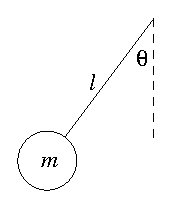
\includegraphics[width=0.15\textwidth]{ode/introduction/pendulum}
  \end{center}
  \caption{A pendulum.}
  \label{figure pendulum}
\end{figure}

Consider the motion of a pendulum in a plane.  
(See Figure~\ref{figure pendulum}.)  The head of the pendulum has mass $m$.
The rod is massless and has length $l$.  Let $\theta$ be the angular displacement
from the vertical resting position.  The angular velocity is $\dot{\theta}$.
The angular momentum is $l^2 m \dot{\theta}$.  The pendulum moves under the 
force of gravity, $g$ in the downward direction.  This produces a 
torque of $- l m g \sin \theta$.  We equate the torque with the derivative 
of the angular momentum to obtain the differential equation of the 
motion.
\begin{gather*}
  \frac{ \dd }{ \dd t } ( l^2 m \dot{\theta} ) = - l m g \sin \theta
  \\
  \ddot{\theta} + \frac{g}{l} \sin \theta = 0
\end{gather*}
For small $\theta$, $\sin \theta \approx \theta$.  Thus for small oscillations, the motion 
is approximately modelled by an equation for simple harmonic motion:
\[
\ddot{\theta} + \frac{g}{l} \theta = 0.
\]
The frequency for small oscillations is $\omega \approx \sqrt{ g / l }$.


%% CONTINUE





\raggedbottom
%%============================================================================
\exercises{
\pagebreak
\flushbottom
\section{Exercises}




\raggedbottom
}
%%============================================================================
\pagebreak
\flushbottom
\section{Hints}
\hints{

\begin{Hint}
  \label{hint mass on spring solutions}
  Use a trigonometric identity (Appendix~\ref{trigonometric_identities}) 
  to show that the solutions are equivalent.
\end{Hint}

\begin{Hint}
  \label{hint hunter monkey}
  This is a 2-D problem.  The bullet and the monkey move in the vertical 
  plane defined by the hunter and the initial position of the monkey.  Let 
  the hunter be at the origin and fire the rifle at $t = 0$.  Let the 
  initial position of the monkey be a distance $d$ from the hunter and
  and angle $\theta$ from the horizontal axis.  Let the bullet travel with 
  a speed of $v$.  Let $(x,y)$ be the
  position of the bullet and $(\xi,\psi)$ be the position of the monkey.
  Find the positions as a function of time and then see if there
  is a solution of $(x(t), y(t)) = (\xi(t), \psi(t))$ for some positive time.
\end{Hint}





\raggedbottom
}
%%============================================================================
\pagebreak
\flushbottom
\section{Solutions}
\solutions{

\begin{Solution}
  \label{solution mass on spring solutions}
  Consider the first proposed solution.
  \begin{gather*}
    x = a \cos( \omega_0 t ) + b \sin( \omega_0 t )
    \\
    \ddot{x} = - a \omega_0^2 \cos( \omega_0 t ) - b \omega_0^2 \sin( \omega_0 t )
  \end{gather*}
  We substitute it into the differential equation and obtain an identity.
  \begin{gather*}
    \ddot{x} + \omega_0^2 x = 0
    \\
    \left( - a \omega_0^2 \cos( \omega_0 t ) - b \omega_0^2 \sin( \omega_0 t ) \right)
    + \omega_0^2 \left( a \cos( \omega_0 t ) + b \sin( \omega_0 t ) \right) = 0
    \\
    0 = 0
  \end{gather*}

  Likewise with the second proposed solution.
  \begin{gather*}
    x = A \sin( \omega_0 t + \phi )
    \\
    \ddot{x} = - A \omega_0^2 \sin( \omega_0 t + \phi )
  \end{gather*}
  We substitute it into the differential equation and obtain an identity.
  \begin{gather*}
    \ddot{x} + \omega_0^2 x = 0
    \\
    \left( - A \omega_0^2 \sin( \omega_0 t + \phi ) \right)
    + \omega_0^2 \left( A \sin( \omega_0 t + \phi ) \right) = 0
    \\
    0 = 0
  \end{gather*}

  The two solutions are equivalent.  To demonstrate this 
  we use trigonometric identities
  to change the form of the second solution.
  \[
  A \sin( \omega_0 t + \phi ) 
  = A \sin \phi \cos( \omega_0 t ) + A \cos \phi \sin( \omega_0 t )
  \]
  By equating the two solutions we see how the parameters are related.
  \[
  a = A \sin \phi, \quad b = A \cos \phi
  \]
  We can also write $A$ and $\phi$ in terms of $a$ and $b$.
  First we square and add the equations to determine $A$.
  \begin{gather*}
    a^2 + b^2 = A^2 (\sin^2 \phi + \cos^2 \phi)
    \\
    A = \sqrt{ a^2 + b^2 }
  \end{gather*}
  Then we determine $\phi$.
  \begin{gather*}
    b = \sqrt{ a^2 + b^2 } \cos \phi
    \\
    \phi = \arccos \left( \frac{ b }{ \sqrt{ a^2 + b^2 } } \right)
  \end{gather*}
\end{Solution}





\begin{Solution}
  \label{solution hunter monkey}
  This is a 2-D problem.  The bullet and the monkey move in the vertical 
  plane defined by the hunter and the initial position of the monkey.  Let 
  the hunter be at the origin and fire the rifle at $t = 0$.  Let the 
  initial position of the monkey be a distance $d$ from the hunter and
  and angle $\theta$ from the horizontal axis.  Let the bullet travel with 
  a speed of $v$.  We assume the speed is sufficient for the bullet to 
  reach the monkey before either hits the ground.  Let $(x,y)$ be the
  position of the bullet and $(\xi,\psi)$ be the position of the monkey.
  We will find the positions as a function of time and then see if there
  is a solution of $(x(t), y(t)) = (\xi(t), \psi(t))$.

  First we write the differential equations and the initial conditions.
  (We know that $\xi(t) = d \cos \theta$ because the monkey falls vertically.)
  \begin{gather*}
    \ddot{x} = 0, \quad x(0) = 0,\ \dot{x}(0) = v \cos \theta
    \\
    \ddot{y} = - g, \quad y(0) = 0,\ \dot{y}(0) = v \sin \theta
    \\
    \ddot{\psi} = - g, \quad y(0) = d \sin \theta,\ \dot{y}(0) = 0
  \end{gather*}
  We can solve the differential equation for $x$ by integrating.
  \begin{gather*}
    \ddot{x} = 0
    \\
    \int_0^t \ddot{x}(\tau) \,\dd \tau = 0
    \\
    \dot{x}(t) - \dot{x}(0) = 0
    \\
    \dot{x}(t) = v \cos \theta
    \\
    \int_0^t \dot{x}(\tau) \,\dd \tau = \int_0^t v \cos \theta \,\dd \tau
    \\
    x(t) - x(0) = v t \cos \theta
    \\ 
    x(t) = v t \cos \theta
  \end{gather*}
  Equation~\ref{equation 1D trajectory solution} gives the solution for
  $y(t)$ and $\psi(t)$.
  \begin{gather*}
    y(t) = - \frac{g}{2} t^2 + v t \sin \theta
    \\
    \psi(t) = - \frac{g}{2} t^2 + d \sin \theta
  \end{gather*}

  Now we determine if there is a time when the positions of the bullet and
  the monkey coincide.  First we solve for the horizontal position.
  \begin{gather*}
    x(t) = \xi(t)
    \\
    v t \cos \theta = d \cos \theta
    \\
    t = \frac{d}{t}
  \end{gather*}
  Then we solve for the vertical position.
  \begin{gather*}
    y(t) = \psi(t)
    \\
    - \frac{g}{2} t^2 + v t \sin \theta = - \frac{g}{2} t^2 + d \sin \theta
    \\
    t = \frac{d}{t}
  \end{gather*}
  Thus we see that the bullet hits the monkey at $t = d / v$.
\end{Solution}


\raggedbottom
}